\section{Theorie}
\subsection{Tunneleffekt}
Die Funktionsweise des Rastertunnelmikroskops basiert auf dem quantenmechanischen Phänomen des Tunneleffekts. Ist ein Wellenpaket von einer endlich hohen Potentialbarriere eingeschlossen, kann es diese im klassischen Fall nicht durchdringen. Quantenmechanisch ist dies jedoch möglich, da das Wellenpaket durch eine Lösung der Schrödingergleichung beschrieben werden kann, die im Betragsquadrat lediglich Information über die Aufenthaltswahrscheinlichkeit des Wellenpakets liefert. Diese Wahrscheinlichkeit ist außerhalb der Potentialbarriere ungleich null, sodass das Wellenpaket durchaus hinter der Barriere auffindbar sein kann. 

\noindent Bei der STM wird ein elektrisch leitender oder mit einem solchen Material überzogener Festkörper untersucht, indem eine leitende Drahtspitze an eine Probe genähert wird, die dann über diese rastert. Die zu überwindende Potentialbarriere für den Tunneleffekt in diesem Versuch ist Luft. Der Effekt ist nur für Abstände in atomarer Skala relevant, weswegen der Versuchsaufbau sensitiv gegenüber dem Abstand zwischen Spitze und Probe ist.

\noindent Wird eine Spitze in die Nähe einer Probe gebracht, kann der Tunneleffekt für die Elektronen der Spitze oder für die der Probe eintreten, was davon abhänging ist, welches Vorzeichen die zwischen Probe und Spitze angelegte Spannung hat. Es entsteht ein Tunnelstrom, der gemessen werden kann.

\noindent Die Sensitivität gegenüber dem Abstand wird in der Formel \eqref{strom} dargestellt. Darin fällt der Strom exponentiell mit dem Abdstand \(d\) .

\begin{equation} 
\label{strom}
I_\text{T}=\frac{U}{d}\exp{(-Kd\sqrt{\Phi})},\quad K\approx1,025\frac{1}{\text{\r{A}}\text{eV}^\frac12}
\cite{hopg}
\end{equation}

\noindent Daraus ergeben sich direkt die zwei Hauptschwierigkeiten dieses Versuchs. Zum einen muss der gesamte Versuchsaufbau bezüglich mechanischer Vibrationen in der Größenordnung von \(<1\)\,\r{A} gedämpft werden, da der Abstand \(d\approx0,5\)\,\r{A} \cite{hopg} anfällig auf sehr schwache Schwingungen ist.  

\noindent Zum anderen muss die Drahtspitze möglichst spitz und sauber präpariert sein.

\noindent Da es bei der STM zwei Modi gibt, einmal die Variation des Abstandes und das konstant Halten des Tunnelstroms und einmal die Variation des Stromes und das konstant Halten des Abstandes, wobei letzteres als Rasterkraftmikroskopie bekannt ist, für welche die Van-der-Waals-Kraft sowie die repulsive Wechselwirkung eine Rolle spielen, soll auf diese noch kurz eingegangen werden.
 
\subsection{Bindungstypen in Kristallen}
\subsubsection{Van-der-Waals-Wechselwirkung}
Diese Kraft ist relativ schwach und wird erst bei einer großen Anzahl von Atomen relevant. Sie entsteht durch ein gegenseitig induziertes Dipolmoment als Wirkung von Fluktuationen in der Ladungsverteilung der Atome. Das rührt daher, dass die Ladungsverteilung nicht starr ist.

\noindent Die Kraft fällt mit der negativ reziproken sechsten Potenz des Abstandes und ist somit sensitiv gegenüber Schwankungen.

\subsubsection{Repulsive Wechselwirkung}
Wird die Spitze zu nah an die Probe gefahren, tritt eine abstoßende Kraft zwischen Spitze und Probe ein. Diese wird repulsive Wechselwirkung genannt. Sie entsteht durch das Überlappen der Elektronenladungsverteilungen unter Berücksichtigung des Paulischen Ausschließungsprinzips.

\noindent Ein empirisch abgeleitetes Potential, welches die Herkunft dieser Kraft beschreibt, ist das Lennard-Jones-Potential \cite{kittel}.

\begin{equation}
U_\text{LJ}(R)=4\epsilon\left[\frac{\sigma}{R}^{12}-\frac{\sigma}{R}^6\right]
\end{equation}

\noindent Hierbei ist \(R\) der Abstand, \(\epsilon\) ein Skalierungsfaktor, der die Stärke der Wechselwirkung beschreibt und \(\sigma\) der Abstand, bei dem das Lennard-Jones-Potential zwischen anziehend und abstoßend wechselt.

\subsection{Fehlerquellen}
\label{kap2}

\noindent Bei diesem Versuch entstehen die Messunsicherheiten überwiegend aus den Eigenschaften von Piezokristallen. In diesem Kapitel werden die unterschiedlichen Fehlerquellen erläutert.

\subsubsection{Intrinsische Nichtlinearität}
Liegt eine Spannung an einem Piezokristall, ändert sich dessen Länge. Diese Änderung ist allerdings nicht linear, wie die gestrichelte Linie in Abbildung \ref{fig:nichtlinearität}.  

\begin{figure}
	\centering
		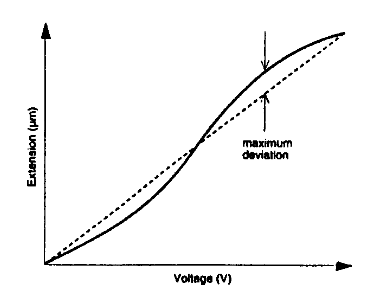
\includegraphics[width=0.5,scale=0.75\textwidth]{nichtlinearitat.png}
	\caption{Längenänderung über Spannung}
	\label{fig:nichtlinearität}
\end{figure}

\noindent Die intrinsische Nichtlinearität ist ein Maß für die maximale Abweichung von der linearen Ausdehnung des Piezokristalls bei gegebener Spannung. 

\noindent Dieser Effekt spiegelt sich bei der Abtastung wider, da die Messpunkte nicht mehr im gleichen Abstand sind und deswegen eine gewisse Verzerrung auftritt.

\subsubsection{Hysterese}
Bei der Ausdehnung eines Piezokristalls unter Anlegen einer Spannung tritt Hysterese auf.
Das bedeutet für die Messung, dass bei einer Bewegung der Spitze in positiver X-Richtung andere Werte gemessen werden als in negativer X-Richtung.

\subsubsection{Kriechen}
Die Reatkion des Piezokristalls auf eine Spannungsänderung findet im Idealfall instantan statt.
In der Realität lässt sich die Bewegung in zwei Teile aufteilen.
Der erste Teil der Bewegung findet in weniger als einer Millisekunde statt, während der zweite Teil länger dauert.
Der Kriechfaktor gibt das Verhältnis der Strecken vom ersten und zweiten Teil an.

Eine Folge dieses Effekts ist, dass Messungen, die mit unterschiedlicher Geschwindigkeit durchgeführt werden, unterschiedliche Ergebnisse liefern können.

\subsubsection{Alterung}
Die Ausrichtung der Dipole im Piezokristall wird durch Anlegen von Spannung beeinflusst.
Ebenso hebt sich die Ausrichtung der Dipole bei längerer Lagerung auf.
Als Folge davon ändert sich der Belastungskoeffizient des Piezokristalls und die Position auf der X, Y und Z-Achse wird verfälscht.

\subsubsection{Kreuzkopplung}

Die Spitze ist an einem Röhren-Piezo angebracht.
Das Strecken der Röhre führt nicht, wie gewünscht, zu einer Translationsbewegung auf einer Achse, sondern zu einer Art Schwenkbewegung auf mehreren Achsen.
Die ungewünschte Bewegung entlang der anderen Achsen wird als Kreuzkopplung bezeichnet.

Die Kreuzkopplung wird entweder durch Software korrigiert oder die Spitze wird durch eine Regelschleife an die korrekte Stelle gefahren.

\subsubsection{Thermische Effekte}
Erwärmung und Abkühlung der Messspitze bzw. der Probe können den Tunnelstrom verändern und somit die Messung verfälschen.
Deshalb sollten die Spitze und Probe nicht berührt werden.
Außerdem wird ein Glasgefäß über das Mikroskop gestülpt, um Luftaustausch zu vermeiden.

\subsection{PID-Regelschleife}
Beim Rastern der Probe wird der Abstand zwischen Probe und Spitze (Z-Achse) variiert und der Tunnelstrom konstant gehalten.
Dies passiert mit einer PID-Regelschleife.
Dabei wird ein Fehlersignal, in diesem Fall die Differenz zwischen dem tatsächlichen und dem gewünschten Tunnelstrom, minimiert.
Das Signal, das der PID-Regler generiert, setzt sich aus drei Komponenten zusammen. Eine Komponente ist proportional zum Fehlersignal, eine ist proportional zum Integral und eine ist proportional zur Ableitung.
Die Eigenschaften des PID-Reglers können angepasst werden, indem die Gewichtungsfaktoren der P-, I-, und D-Komponente verändert werden.